% Translated from: thesis/chapter_04_系统设计与实现.md
% Target journal: General
% Generated: 2026-04-03

% --- Paragraph 1 ---
% # 第四章 系统设计与实现

\chapter{System Design and Implementation}
\setcounter{figure}{0}
\setcounter{equation}{0}
\renewcommand{\thefigure}{\thechapter-\arabic{figure}}
\renewcommand{\theequation}{\thechapter-\arabic{equation}}

% --- Paragraph 2 ---
% ## 4.1 系统总体架构

\section{Overall System Architecture}

% --- Paragraph 3 ---
% 从整体上看，本文实现的实验系统可划分为规则解析层、状态机层、搜索代理层、状态编码与价值评估层，以及实验编排与结果归档层五个部分。规则解析层负责将 GDL/KIF 规则描述转化为可执行的逻辑表示；状态机层在统一接口下提供角色读取、初始状态生成、合法动作查询、状态转移、终局判定与得分获取；搜索代理层在共享 MCTS 内核上实现纯搜索、启发式搜索与神经价值增强搜索；状态编码与价值评估层负责将局面表示为模型输入，并输出对非终局状态的价值估计；实验编排与结果归档层则负责完成数据构建、模型训练、在线对局评测以及实验结果留档。

The experimental system in this thesis is organized into five layers: rule parsing, state machine, search agent, state encoding and value evaluation, and experiment orchestration with result archiving. The rule-parsing layer converts GDL/KIF descriptions into executable logical representations. The state-machine layer provides unified interfaces for role retrieval, initial-state construction, legal-action query, state transition, terminal detection, and goal-value query. The search-agent layer implements pure search, heuristic search, and neural-value-enhanced search on a shared MCTS kernel. The encoding-and-evaluation layer maps game states to model inputs and outputs value estimates for non-terminal states. The orchestration-and-archiving layer manages data construction, model training, online match evaluation, and experiment logging.

% --- Paragraph 4 ---
% 这种分层结构的直接好处在于，不同模块之间通过稳定接口协同，而不是通过相互穿透的方式耦合。规则表示的变化不会破坏搜索框架，价值模型的替换也不需要改写状态机逻辑；当研究需要增加新的对比方法或新的实验口径时，通常只需在实验编排层调整配置与流程，而无需重构底层执行内核。对于本文而言，这说明研究对象并不是一段孤立算法，而是一套围绕 SDRPV 方法构建的完整实验系统。

The direct benefit of this layered design is stable collaboration through explicit interfaces rather than cross-module entanglement. Changes in rule representation do not break the search framework, and replacing value models does not require rewriting state-machine logic. When new baselines or evaluation protocols are added, updates are typically limited to the orchestration layer. For this paper, this shows that the research object is not an isolated algorithm, but a complete experimental system built around the SDRPV method.
Figure~\ref{fig:system_architecture} visualizes this five-layer organization and the main data/control flow across layers.

% --- Paragraph 5 ---
% 【图 4-1 预留：系统总体架构图。建议展示“规则描述层 -> 统一状态机 -> MCTS 搜索代理 -> 状态编码与价值评估 -> 实验编排与结果归档”的数据流与调用关系。】

\begin{figure}[htbp]
\centering
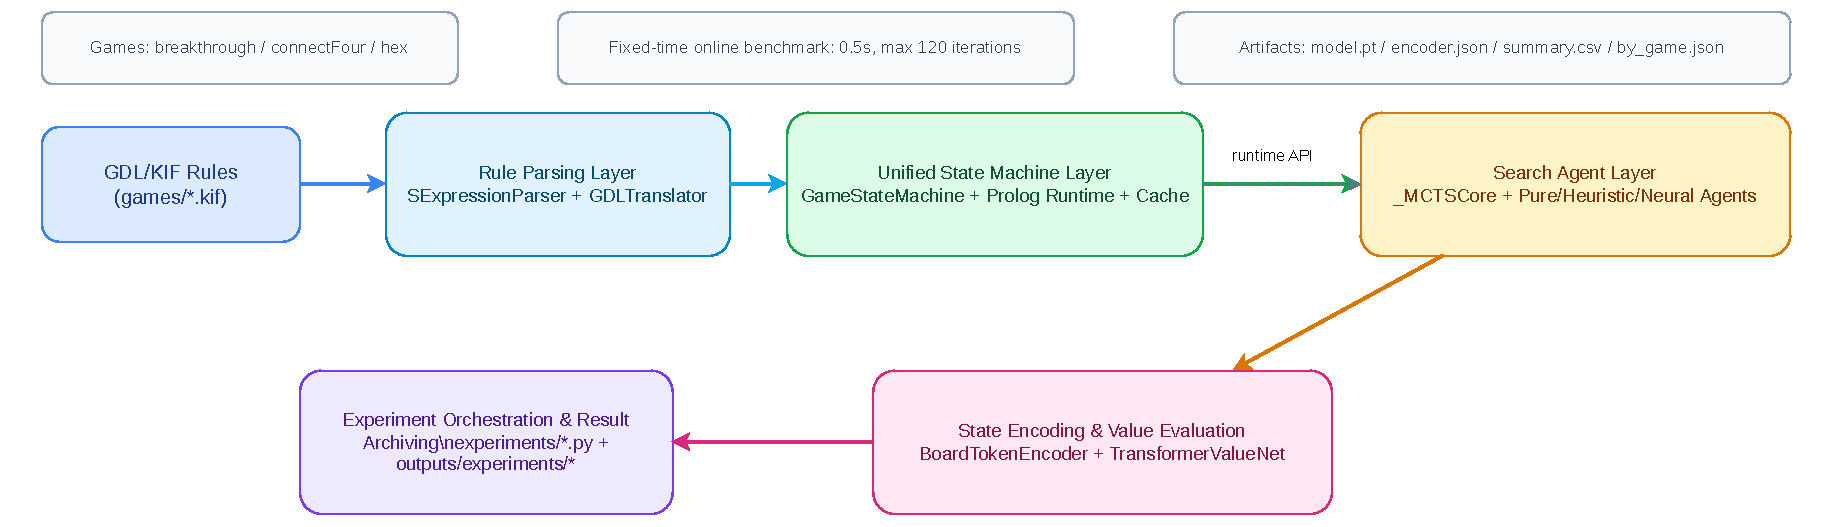
\includegraphics[width=0.92\linewidth]{img/system_architecture.pdf}
\caption{Overall system architecture.}
\label{fig:system_architecture}
\end{figure}

% --- Paragraph 7 ---
% 为便于读者理解系统组织方式，可进一步将其概括为三类核心对象：一是与游戏规则执行相关的运行对象，二是与搜索和评估相关的算法对象，三是与训练、评测和留档相关的实验对象。这样的组织方式既服务于工程实现，也服务于论文中的证据追踪，因为每一类结论都可以追溯到对应的模块职责、输入输出及其运行阶段。
For clarity, the system can be grouped into three categories of core objects: runtime objects for rule execution, algorithm objects for search and evaluation, and experiment objects for training, benchmarking, and archiving. This organization supports both engineering implementation and evidence traceability.
Table~\ref{tab:system_module_responsibilities} summarizes each module's main input, output, and role in this layered architecture.

% --- Paragraph 8 ---
% 【表 4-1 预留：系统模块职责说明表。建议列出规则解析、状态机、搜索代理、状态编码、价值评估、实验编排、结果归档等模块的主要输入、输出和作用。】

\begin{table}[htbp]
\centering
\caption{Responsibilities of system modules}
\label{tab:system_module_responsibilities}
\begin{tabular}{p{2.0cm}p{3.2cm}p{3.0cm}p{4.1cm}}
\toprule
Module & Main input & Main output & Main role \\
\midrule
Rule parsing & GDL/KIF rule text & Executable representation, intermediate forms & Parsing, syntax translation, and reasoning preparation \\
State machine & Rule IR, current state, joint action & Legal actions, next state, terminal status, goal value & Unified game-execution interface across games \\
Search agent & State-machine API, budget, evaluator config & Selected action, search-tree statistics & Pure, heuristic, and neural-enhanced search on shared MCTS \\
State encoding & State facts, position indices, stage features & Token sequences, masks, global-feature tensors & Unified cross-game neural input mapping \\
Value evaluation & Encoded state, model parameters & Scalar value estimate & Neural evaluation for non-terminal leaf nodes \\
Experiment orchestration & Data config, training tasks, benchmark tasks & Training runs, benchmark outputs & End-to-end control of data, training, and online evaluation \\
Result archiving & Metadata, match logs, metrics & Summary tables, model artifacts, archived files & Reproducibility, comparison analysis, and traceability \\
\bottomrule
\end{tabular}
\end{table}


% --- Paragraph 10 ---
% ## 4.2 通用规则解析与状态机实现
\section{Unified Rule Parsing and State-Machine Implementation}

% --- Paragraph 11 ---
% 在 GGP 场景下，首先需要解决的问题不是如何训练价值模型，而是如何让不同游戏在统一程序接口上被执行。为此，系统采用“规则解析 + 统一状态机”的两阶段实现思路：先将 GDL/KIF 规则文本解析为结构化表达，再转写为逻辑推理可直接处理的中间表示，从而使不同游戏都能够在同一求解框架中完成推理、对局与搜索。
In GGP, the first problem is not value-model training but unified execution of different games under one program interface. The system adopts a two-stage route: rule parsing plus unified state machine. GDL/KIF rules are parsed into structured forms and then translated into logic-executable intermediate representations, allowing different games to be reasoned and executed under one framework.


% --- Paragraph 12 ---
% 在规则具备可执行性之后，统一状态机负责向上层算法提供标准化接口，包括角色集合读取、初始状态生成、合法动作集合查询、动作联合后的状态转移、终局判断和目标值计算等操作。若将当前状态记为 $s_t$、合法动作集合记为 $\mathcal{A}(s_t)$、联合动作记为 $a_t$，则状态机提供的核心语义可抽象为
After rules become executable, the unified state machine exposes standardized interfaces for role retrieval, initial-state generation, legal-action query, transition execution, terminal checking, and goal evaluation. Let $s_t$ be current state, $\mathcal{A}(s_t)$ legal actions, and $a_t$ a joint action. The core semantics are

\begin{equation}
a_t \in \mathcal{A}(s_t),\qquad s_{t+1}=T(s_t,a_t),\qquad r_t=R(s_t),
\end{equation}


% --- Paragraph 14 ---
% 其中 $T(\cdot)$ 表示状态转移函数，$R(\cdot)$ 表示终局得分函数。对搜索算法而言，这种统一接口非常关键，因为它使纯搜索基线、启发式搜索基线和神经价值增强方法都建立在相同的环境语义之上，避免了“不同方法实际上比较的是不同执行环境”的问题。
where $T(\cdot)$ is transition and $R(\cdot)$ is terminal scoring. This interface is essential because pure-search baselines, heuristic-search baselines, and neural-value-enhanced methods all run on the same environment semantics. It avoids the problem that different methods actually compare different execution environments.

% --- Paragraph 15 ---
% 考虑到 MCTS 在同一局面附近会反复访问相邻节点，系统还在状态机内部对高频查询结果进行缓存，以降低重复逻辑推理带来的额外开销。这样做的意义并不仅仅在于提高运行速度，更在于保证固定时间预算下各方法都能够将更多计算资源用于真实搜索，而不是消耗在重复的规则求值上。
To reduce repeated logical-inference overhead near frequently revisited states, the system caches high-frequency query results inside the state machine. The significance of this is not only to improve the running speed, but also to ensure that each method can use more computing resources for real search under a fixed time budget, rather than consuming repeated rule evaluations.


% --- Paragraph 16 ---
% 在本文的实验设置中，\texttt{breakthrough}、\texttt{connectFour} 和 \texttt{hex} 三个游戏虽然规则不同，但都通过这一统一状态机完成执行。因此，跨游戏实验的可行性来自规则层与搜索层之间清晰的接口约束，而不是来自针对单个游戏的专门实现。
In our experiments, \texttt{breakthrough}, \texttt{connectFour}, and \texttt{hex} are all executed through this unified state machine despite rule differences. Cross-game comparability therefore comes from interface constraints between rule and search layers, not game-specific implementations.
Figure~\ref{fig:rule_state_machine_class_diagram} summarizes the key component dependencies, including parser/translator flow, state-machine APIs, and runtime cache support.


% --- Paragraph 17 ---
% 【图 4-2 预留：规则解析与状态机类图。建议以类图形式展示“规则解析器”“规则中间表示”“统一状态机”“缓存组件”之间的依赖关系，以及状态机向搜索层提供的核心接口。】
\begin{figure}[htbp]
\centering
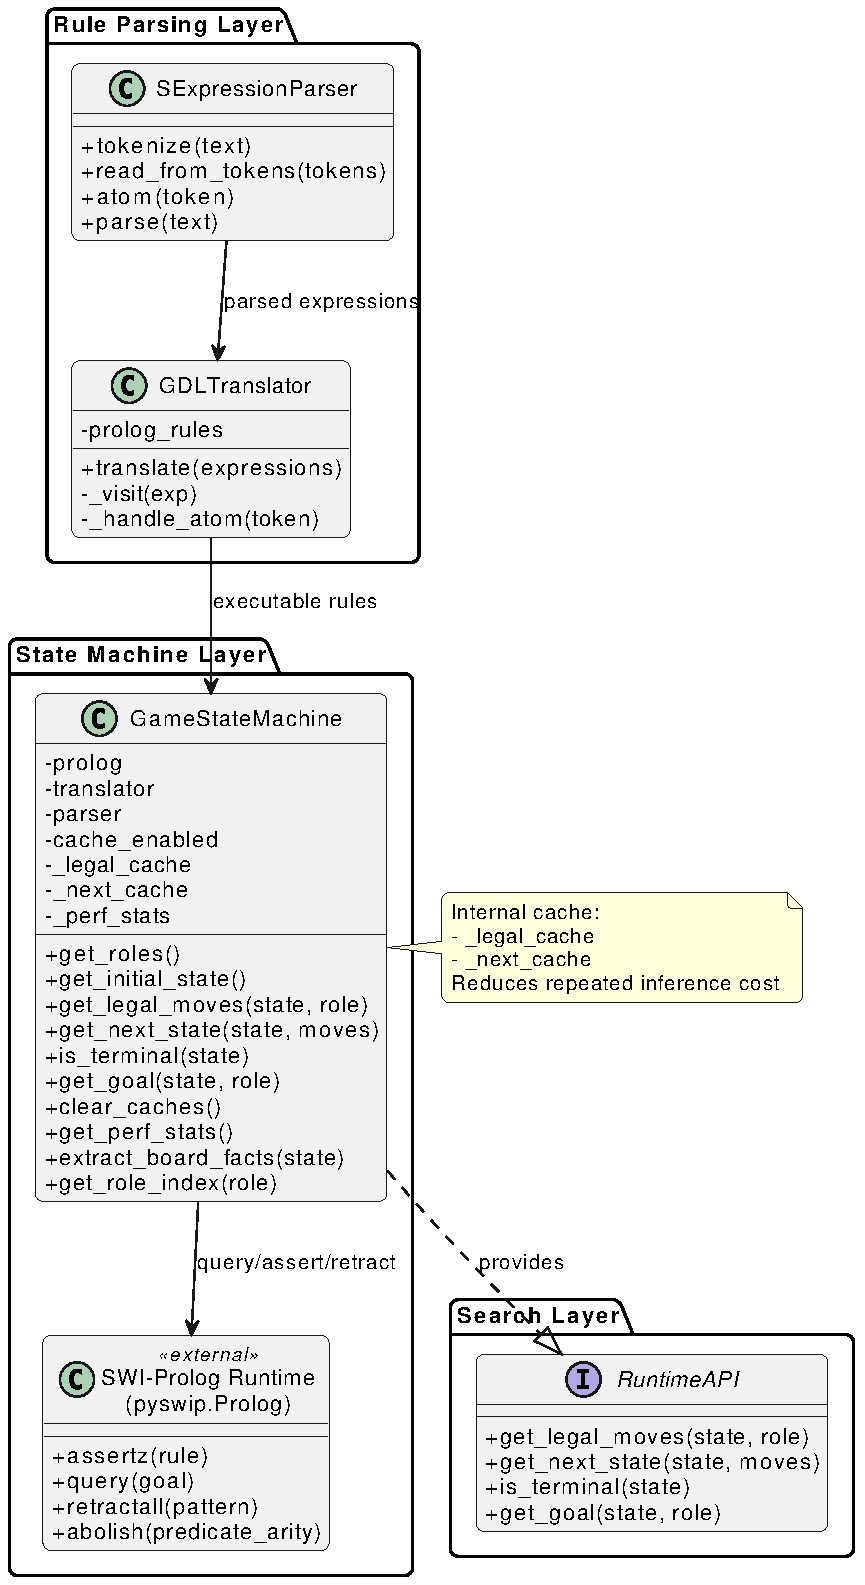
\includegraphics[width=0.90\linewidth]{img/rule_state_machine_class_diagram.pdf}
\caption{Class diagram of rule parsing and state-machine components.}
\label{fig:rule_state_machine_class_diagram}
\end{figure}


% --- Paragraph 19 ---
% ## 4.3 MCTS 内核与搜索代理实现
\section{MCTS Kernel and Search-Agent Implementation}


% --- Paragraph 20 ---
% 在搜索层，系统没有为每一种方法分别实现一套完全独立的流程，而是将“选择、扩展、评估、回传”四个步骤封装到统一的 MCTS 内核中，并通过不同评估策略派生出多类搜索代理。这样做的好处在于，不同方法之间的差异被限制在叶节点评估与动作采样策略上，从而使对比建立在相同的搜索骨架之上。
At the search layer, we do not maintain separate fully independent pipelines per method. Instead, selection, expansion, evaluation, and backpropagation are encapsulated in a shared MCTS kernel, and different search agents are instantiated by plugging in different evaluation strategies. This constrains method differences to leaf evaluation and action sampling under the same search skeleton.


% --- Paragraph 21 ---
% 本文在在线实验中采用三类代表性方法。第一类是 \texttt{pure_mct}，其特点是在 UCT 框架下采用随机仿真完成局面评估，可作为最基础的纯搜索基线。若记节点访问次数为 $N(s)$，边访问次数为 $N(s,a)$，累计回报为 $W(s,a)$，则其选择准则可写为
We evaluate three representative methods online. The first is \texttt{pure_mct}, using random simulation under UCT. With node visits $N(s)$, edge visits $N(s,a)$, and accumulated return $W(s,a)$, the selection rule is

\begin{equation}
a^\ast
=
\arg\max_{a\in \mathcal{A}(s)}
\left(
\frac{W(s,a)}{N(s,a)}
+
c\sqrt{\frac{\ln N(s)}{N(s,a)+1}}
\right).
\end{equation}


% --- Paragraph 23 ---
% 其中 $c$ 为探索系数。第二类是 \texttt{heuristic_mcts}，它在共享搜索内核之上引入历史统计驱动的动作采样与 rollout 引导，使搜索能够利用仿真过程中积累的控制知识，提高相较于纯随机搜索的有效性，这与 Finnsson 和 Björnsson 提出的 simulation-based GGP 思路一致 \cite{finnsson2008simulation}。第三类是神经价值增强搜索，它在非终局叶节点调用价值模型，在终局节点仍直接读取规则层真实得分，从而将学习到的价值估计作为搜索评估的补充信息。这种保留树搜索主循环、重点替换叶节点评估与规划组件的组织方式，也与 MuZero 等神经搜索方法所体现出的模块化集成思路一致 \cite{schrittwieser2020muzero,grill2020regularized}。
where $c$ is the exploration coefficient. 
The second is \texttt{heuristic_mcts}, which adds history-guided action sampling and rollout guidance on the same kernel, consistent with simulation-based GGP enhancements \cite{finnsson2008simulation}. The third is neural-value-enhanced search: non-terminal leaf nodes call the value model, while terminal nodes still use rule-grounded true scores. This way of organizing the main cycle of the tree search, focusing on replacing the leaf node evaluation and planning components, is also consistent with the modular integration ideas embodied in neural search methods such as MuZero \cite{schrittwieser2020muzero, grill2020regularized}.


% --- Paragraph 24 ---
% 统一内核的另一个优点，是叶节点评估逻辑可以与搜索主循环解耦。于是，随机 rollout、历史统计引导的 rollout 以及神经价值评估都能够在相同接口下互换，搜索树结构、UCT 选择逻辑和回传过程则始终保持一致。对于论文中的方法比较而言，这种设计能有效降低方法差异被外围实现差异放大的风险。
A key advantage of the shared kernel is decoupling leaf evaluation from the MCTS main loop. Random rollout, history-guided rollout, and neural evaluation become interchangeable through the same interface while tree structure and backpropagation remain unchanged. This design can effectively reduce the risk of method differences being amplified by peripheral implementation differences.
Figure~\ref{fig:search_agent_class_diagram} shows the shared MCTS core and the three agent branches as interchangeable strategy specializations.

% --- Paragraph 25 ---
% 【图 4-3 预留：搜索代理类图。建议展示统一 MCTS 内核作为父类或核心组件，\texttt{pure_mct}、\texttt{heuristic_mcts} 与神经价值增强搜索代理作为不同策略分支，并分别连接随机评估器、历史统计评估器与神经价值评估器。】

\begin{figure}[htbp]
\centering
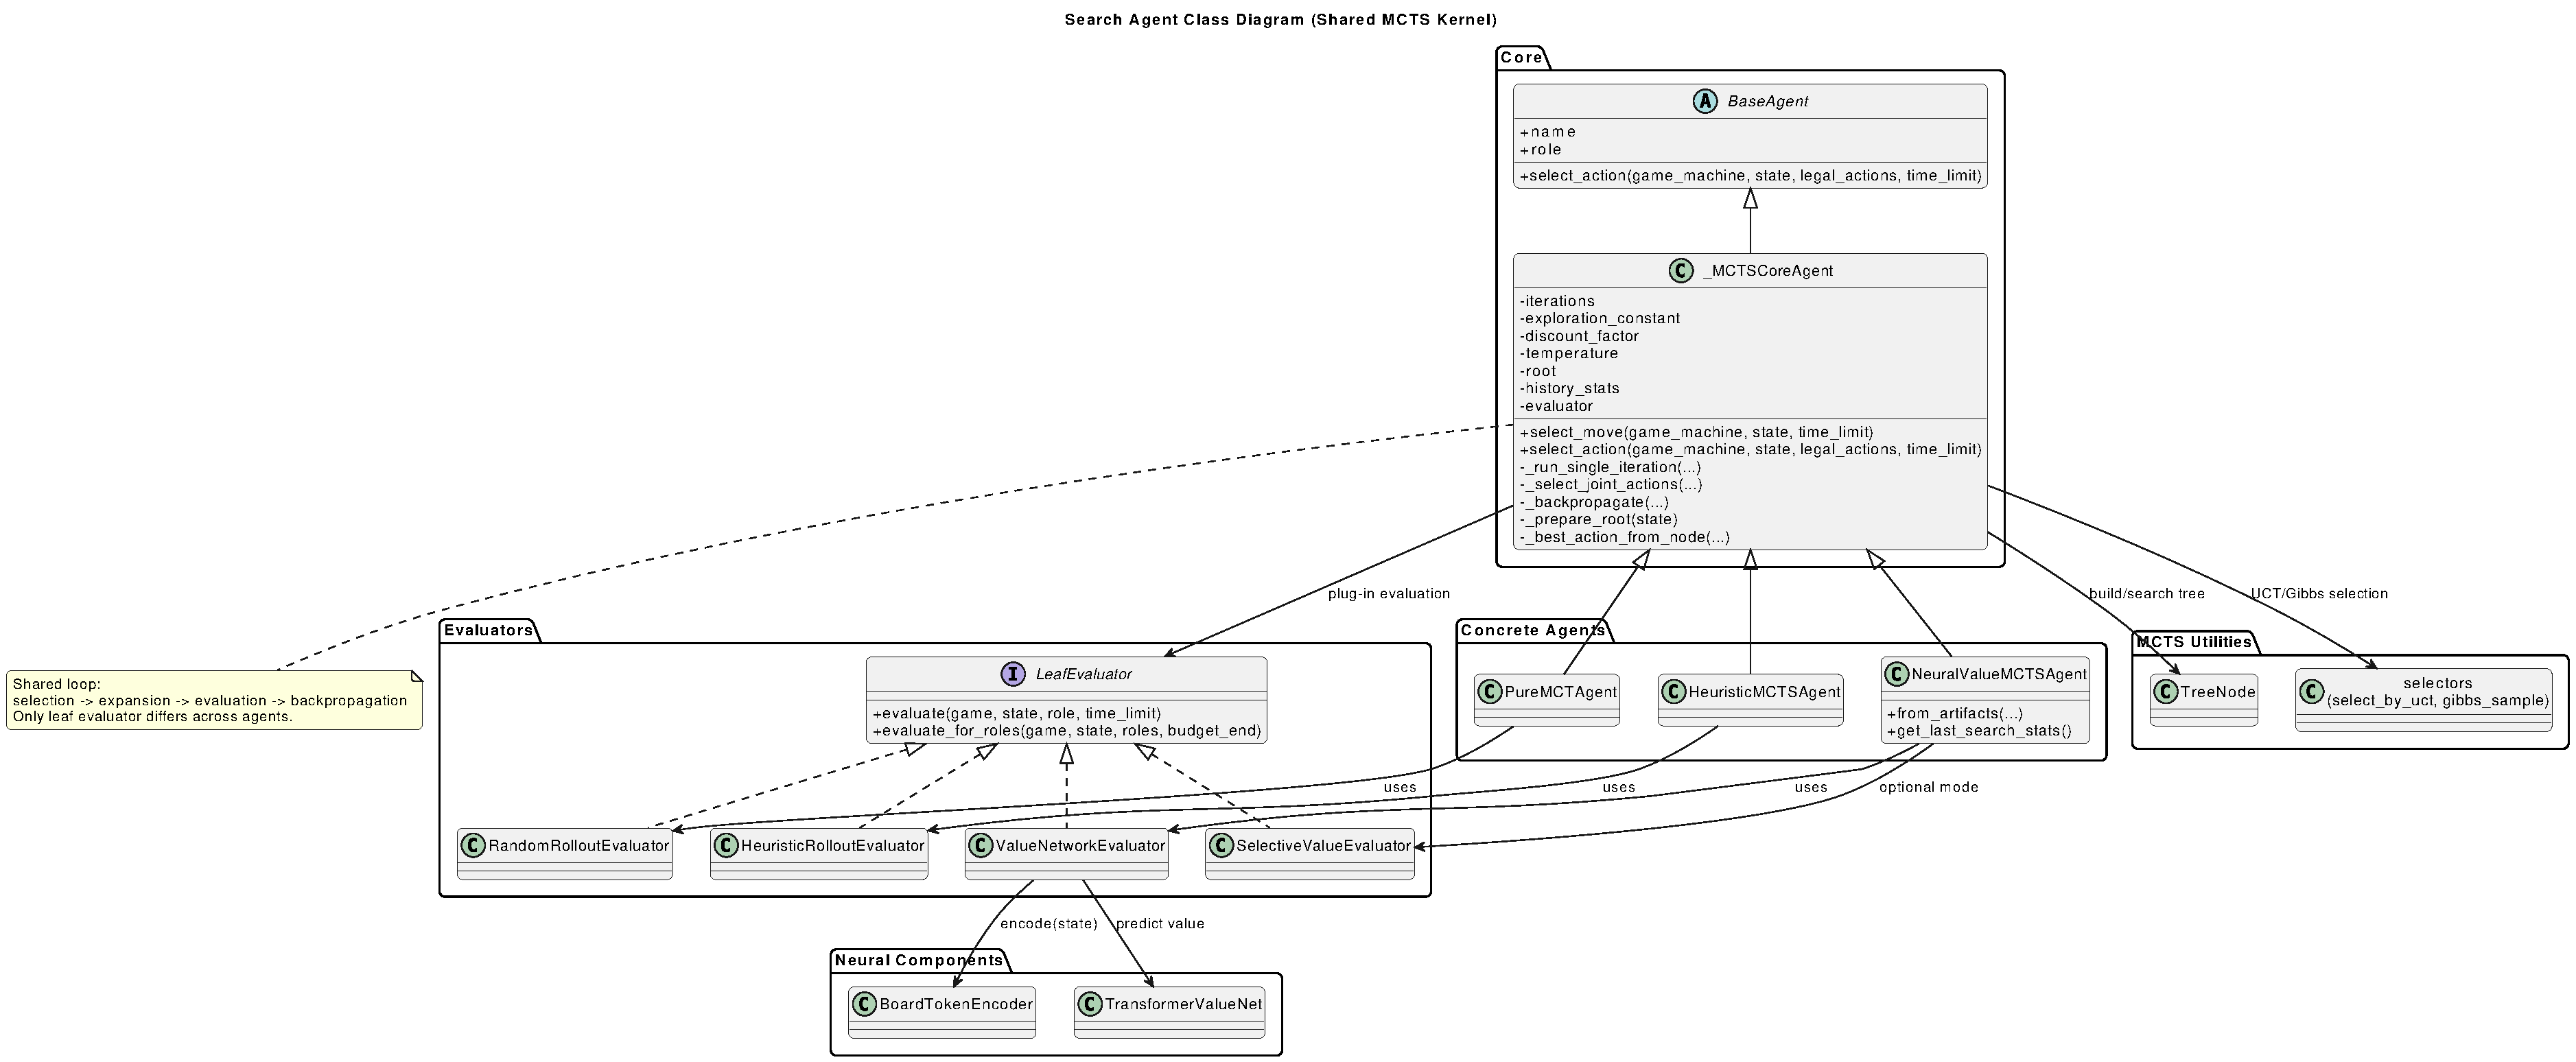
\includegraphics[width=0.92\linewidth]{img/search_agent_class_diagram.pdf}
\caption{Class diagram of search agents.}
\label{fig:search_agent_class_diagram}
\end{figure}


% --- Paragraph 27 ---
% ## 4.4 状态编码、价值网络与推理接口
\section{State Encoding, Value Network, and Inference Interface}


% --- Paragraph 28 ---
% 为了使价值模型同时兼顾 GGP 的统一性和棋盘状态的结构信息，系统采用基于棋盘 token 的状态编码方式。该编码将局面中的棋盘事实拆分为内容标识、位置标识和掩码信息，并辅以行动方、回合阶段和终局标志等全局特征，最终形成适合神经网络处理的张量表示。若棋盘上共有 $n$ 个可观测位置，则编码结果可记为
To preserve both GGP-level generality and board-structure information, we adopt board-token-based state encoding. Board facts are converted into content tokens, position tokens, and masks, together with global features such as acting player, game stage, and terminal flag. If there are $n$ observable positions, encoding is



\begin{equation}
x(s)=\Bigl(\{(c_i,p_i)\}_{i=1}^{n},\ m,\ \phi(s)\Bigr),
\end{equation}

% --- Paragraph 30 ---
% 其中 $c_i$ 表示第 $i$ 个位置的内容 token，$p_i$ 表示其位置编码，$m$ 表示有效位置掩码，$\phi(s)$ 表示全局阶段特征。这样的设计既保留了棋盘游戏的空间结构，又避免了为每一种游戏手工设计不同输入格式。
where $c_i$ is content token, $p_i$ position encoding, $m$ valid-position mask, and $\phi(s)$ stage features. This design not only retains the spatial structure of the board game, but also avoids the manual design of different input formats for each game.


% --- Paragraph 31 ---
% 在模型层，本文采用基于 Transformer 的价值评估结构，并将其作为神经价值搜索的核心评估器。一方面，这一设计能够与 \texttt{baseline_token_transformer} 所代表的神经价值基线保持一致的表示范式，便于在线对比；另一方面，它也为 SDRPV 中的残差学习提供了统一的特征底座。Transformer 主干通过 token 嵌入、位置编码、掩码池化和全局特征融合完成局面表征，最终输出归一化的标量价值估计，其形式可概括为
At the model level, we use a Transformer-based value network as the core evaluator. This keeps representation style aligned with the \texttt{baseline_token_transformer} baseline and supports residual learning in SDRPV. Transformer backbone completes the situation representation through token embedding, position coding, mask pooling and global feature fusion, and finally outputs normalized scalar value estimation, which can be summarized as follows:

\begin{equation}
h(s)=\mathrm{Transformer}\bigl(x(s)\bigr),\qquad
\hat{v}(s)=\tanh(Wh(s)+b).
\end{equation}

% --- Paragraph 33 ---
% 该思路与 Maras 等人关于以 token 序列和注意力结构处理棋盘状态的方向相呼应 \cite{maras2024fast}。
This idea echoes the direction of Maras et al. \cite {maras2024fast} on dealing with the state of the chessboard with token sequence and attention structure.

% --- Paragraph 34 ---
% 在推理接口上，系统始终将规则真值与模型估计明确区分。对于终局状态，评估结果直接由规则层给出；对于非终局状态，则先由统一编码模块生成模型输入，再由价值网络输出标量估计。这种设计保证了神经评估是补充搜索中的叶节点评估，而不是替代规则系统本身，从而使方法的工程边界和理论边界都更加清晰。
On the inference interface, the system always makes a clear distinction between the true value of the rule and the model estimation. For terminal states, the system returns rule-grounded outcomes directly. For non-terminal states, it uses encoded inputs and neural prediction. This keeps neural evaluation as a supplement to leaf-node evaluation, not a replacement of rule semantics.
Figure~\ref{fig:state_encoding_value_pipeline} presents this inference path from state facts to token encoding, Transformer value prediction, and leaf-node evaluation usage in search.

% --- Paragraph 35 ---
% 【图 4-4 预留：状态编码与价值评估流程图。建议展示“局面事实 -> token 化编码 -> Transformer 价值网络 -> 标量价值估计 -> 搜索叶节点评估”的处理链路。】

\begin{figure}[htbp]
\centering
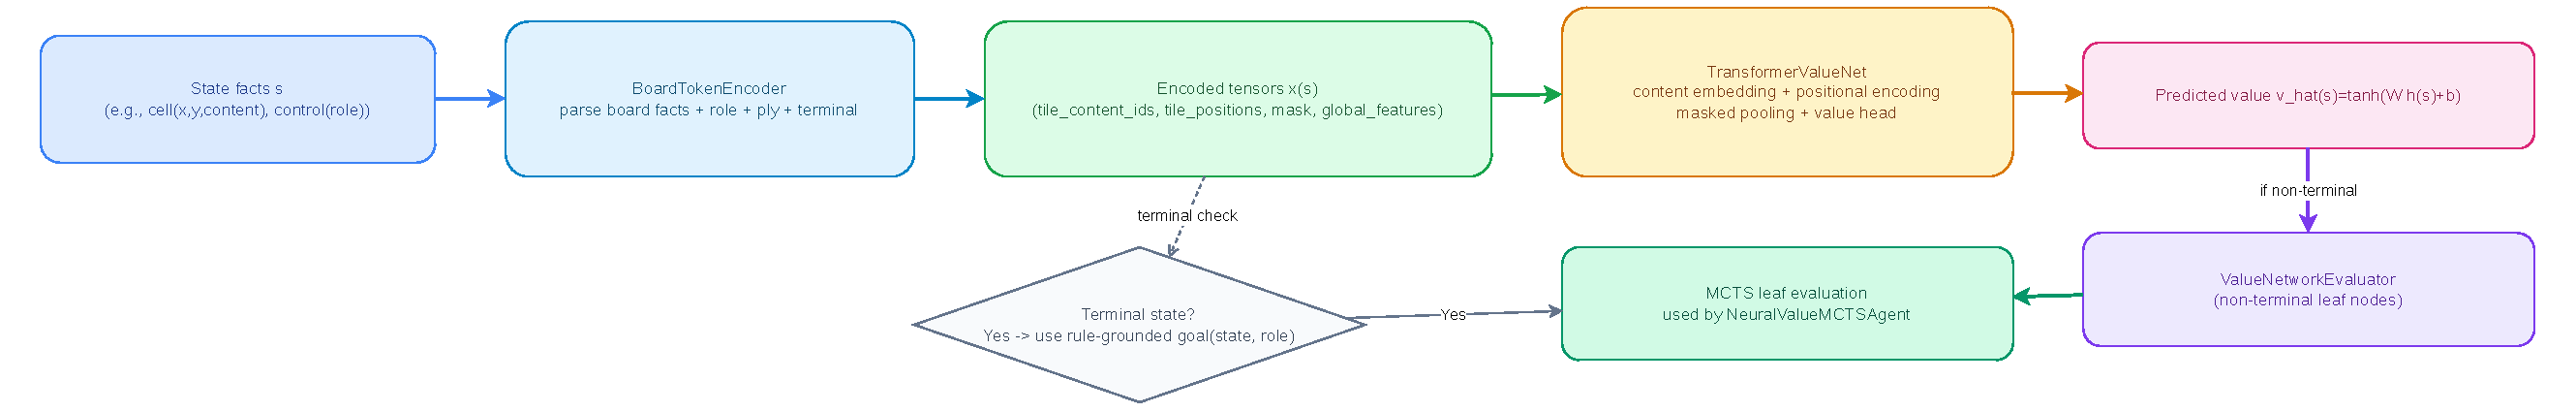
\includegraphics[width=0.92\linewidth]{img/state_encoding_value_pipeline.pdf}
\caption{Pipeline of state encoding and value evaluation.}
\label{fig:state_encoding_value_pipeline}
\end{figure}


% --- Paragraph 37 ---
% ## 4.5 数据构建、模型训练与实验执行链路
\section{Data Construction, Model Training, and Experiment Execution Pipeline}

% --- Paragraph 38 ---
% 本文的训练与评测是一条连续的实验链路。首先，系统采用统一的自对弈与搜索标注流程构建训练样本，将局面状态、低成本基线搜索值、较强搜索值以及必要的上下文信息整理为适合 SDRPV 学习的数据结构。这样做的目的，是让后续模型训练直接围绕“如何在低成本评估基础上学习修正量”这一核心问题展开。
Training and evaluation are organized as one continuous pipeline. First, a unified self-play and search-annotation process constructs samples containing states, low-cost baseline values, stronger-search values, and context features. This allows training to directly target correction over low-cost estimation.


% --- Paragraph 39 ---
% 在模型训练阶段，系统围绕残差目标完成价值模型优化。具体而言，模型并不直接学习终值本身，而是学习相对于基线搜索值的修正量，并通过离线指标持续衡量预测值与较强搜索值之间的一致性，以及相对基线值的误差改善幅度。由此，离线训练与在线部署之间形成了明确对应关系，即离线阶段优化的是更好的叶节点评估，在线阶段检验的是这种评估是否真正提升有限预算下的搜索表现。
During training, the model optimizes residual targets rather than raw final values. Offline metrics track agreement with stronger-search supervision and improvement over baseline estimates. This creates a direct mapping from offline optimization (better leaf evaluation) to online validation (better limited-budget search outcomes).


% --- Paragraph 40 ---
% 在实验执行阶段，系统采用 fixed-time（固定时间）的在线评测口径：每一步决策的搜索时间预算设为 \texttt{0.5 s}，同时将搜索迭代上限设为 \texttt{120} 次。若第 $m$ 步决策的实际搜索时间和搜索迭代数分别记为 $t_m$ 和 $k_m$，则约束可以写为
Online evaluation uses a fixed-time protocol: each move is allocated \texttt{0.5 s} with at most \texttt{120} search iterations. Let per-move runtime and iterations be $t_m$ and $k_m$:


\begin{equation}
t_m \le 0.5,\qquad k_m \le 120.
\end{equation}

% --- Paragraph 42 ---
% 在这一统一预算下，实验分为三类：一是 baseline benchmark，用于比较 SDRPV 方法与 \texttt{pure_mct}、\texttt{heuristic_mcts}、\texttt{baseline_token_transformer} 三个基线在 \texttt{breakthrough}、\texttt{connectFour}、\texttt{hex} 上的真实对局表现；二是 ablation benchmark，用于比较完整方案与不同删减版本之间的性能差异；三是离线指标评测，用于分析残差学习目标是否带来了对较强搜索监督的更好逼近。
Under this unified budget, experiments include three parts: baseline benchmark (SDRPV vs. \texttt{pure_mct}, \texttt{heuristic_mcts}, \texttt{baseline_token_transformer} on \texttt{breakthrough}, \texttt{connectFour}, and \texttt{hex}), ablation benchmark (full model vs. reduced variants), and offline metrics (whether residual objectives better approximate stronger-search supervision).
Table~\ref{tab:training_and_evaluation_pipeline} presents the end-to-end mapping from data construction to online benchmarks, including key inputs, outputs, and the role of each stage.

% --- Paragraph 43 ---
% 【表 4-2 预留：训练与评测链路说明表。建议列出数据构建、残差训练、离线指标评估、baseline benchmark、ablation benchmark 五个阶段的输入、输出和核心作用。】

\begin{table}[htbp]
\centering
\caption{Training and evaluation pipeline}
\label{tab:training_and_evaluation_pipeline}
\begin{tabular}{p{2.5cm}p{3.2cm}p{3.1cm}p{3.8cm}}
\toprule
Stage & Main input & Main output & Core role \\
\midrule
Data construction & Self-play traces, shallow-search values, teacher-search values, terminal scores & Standardized SDRPV samples & Build unified samples with $s,b,q_t,z,\phi,\text{metadata}$ \\
Residual training & Train/validation samples, Transformer value network, residual targets & Trained residual value model & Learn correction over baseline estimates \\
Offline evaluation & Test-set samples, model predictions, baseline values, teacher values & MAE, correlation, error-gain metrics & Verify improvement over baseline toward stronger supervision \\
Baseline benchmark & Trained model, three baseline agents, fixed-time budget & Per-game and overall win rates & Evaluate overall competitiveness in online matches \\
Ablation benchmark & Full and reduced variants under unified settings & Ablation results and deltas & Quantify contributions of teacher supervision and residual objective \\
\bottomrule
\end{tabular}
\end{table}


% --- Paragraph 45 ---
% ## 4.6 结果归档与复现性设计
\section{Result Archiving and Reproducibility Design}


% --- Paragraph 46 ---
% 为了保证实验结论可追溯、可复核，系统对训练阶段和在线评测阶段的产物都采用结构化归档。归档内容包括实验元数据、逐局对局结果、按游戏和配置汇总的统计结果、离线训练指标、模型产物、训练样本以及与实验运行相关的附加工件。通过这种组织方式，论文中的任一关键结论都能够回溯到对应实验的参数、对局记录和统计摘要。
To ensure traceability and reproducibility, both training and online-evaluation artifacts are archived in structured form, including metadata, per-game logs, aggregated statistics, offline metrics, model artifacts, and associated outputs. Any key claim in this thesis can be traced back to concrete configurations and records.

% --- Paragraph 47 ---
% 本文在复现性设计上还遵循了几个原则。第一，所有在线方法共享同一状态机、同一 MCTS 主循环和一致的终局评分规则，使方法差异集中体现在评估策略而非环境实现上。第二，baseline benchmark 与 ablation benchmark 统一采用 fixed-time 口径，即每步 \texttt{0.5 s} 搜索时间预算和 \texttt{120} 次搜索迭代上限，避免不同预算设置引入额外干扰。第三，在线结果均以 \texttt{seed=242} 的实验留档为准，使实验描述、结果统计与后续分析保持一致。第四，终局节点始终直接读取规则真值，避免神经模型对游戏规则产生覆盖。
Reproducibility is enforced through four principles: all methods share the same state machine, MCTS loop, and terminal scoring; baseline and ablation benchmarks use the same fixed-time budget (\texttt{0.5 s} and \texttt{120} iterations); online records are archived with \texttt{seed=242}; and terminal values always come from rule-grounded truth rather than neural overrides.

% --- Paragraph 48 ---
% 这些实现细节共同支撑了本文的实验可信度。换言之，系统设计的目标不仅是跑通实验，更是让实验结论在统一口径下被解释、复核并复现。
These design choices make the goal not only to run experiments successfully, but to ensure that conclusions are interpretable, verifiable, and reproducible under a unified protocol.
